\begin{appendix}

\chapter{Meetings}\label{ch:Meetings}
The following tables show the minutes of most of the team meetings.

\begin{figure}[htbp]
  \centering
    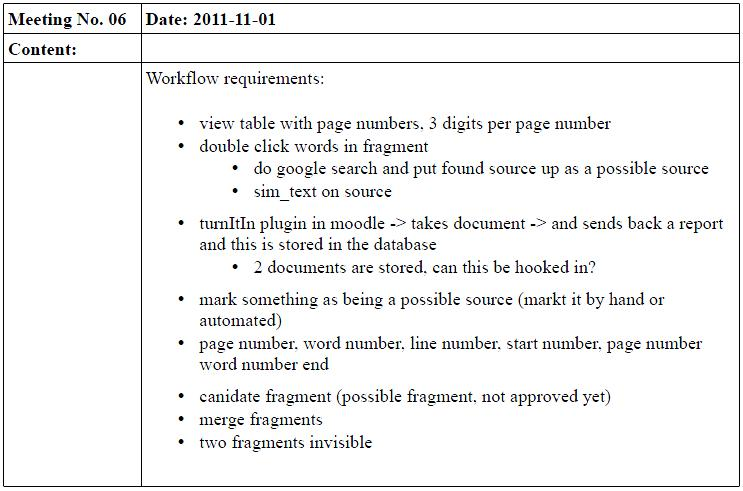
\includegraphics[width=\textwidth]{images/a_meetings/meeting_6}
  \caption{Meeting minutes no. 6}
  \label{fig:meeting minutes no. 6}
\end{figure}

\begin{figure}[htbp]
  \centering
    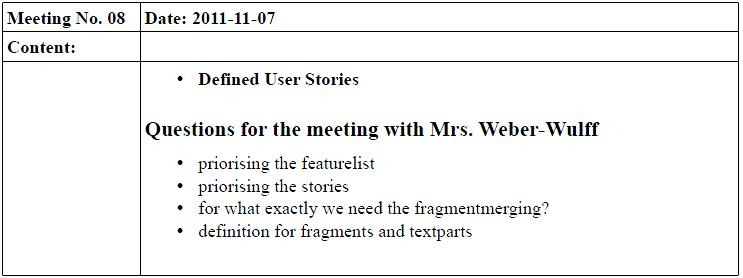
\includegraphics[width=\textwidth]{images/a_meetings/meeting_8}
  \caption{Meeting minutes no. 8}
  \label{fig:meeting minutes no. 8}
\end{figure}

\begin{figure}[htbp]
  \centering
    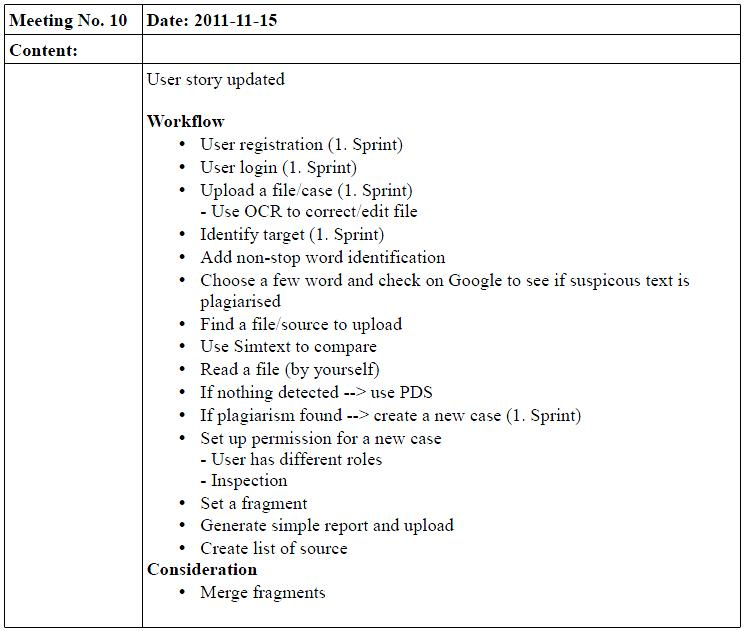
\includegraphics[width=\textwidth]{images/a_meetings/meeting_10}
  \caption{Meeting minutes no. 10}
  \label{fig:meeting minutes no. 10}
\end{figure}

\begin{figure}[htbp]
  \centering
    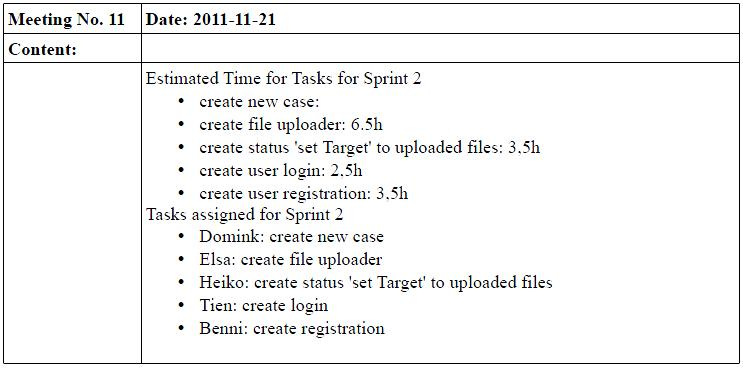
\includegraphics[width=\textwidth]{images/a_meetings/meeting_11}
  \caption{Meeting minutes no. 11}
  \label{fig:meeting minutes no. 11}
\end{figure}

\begin{figure}[htbp]
  \centering
    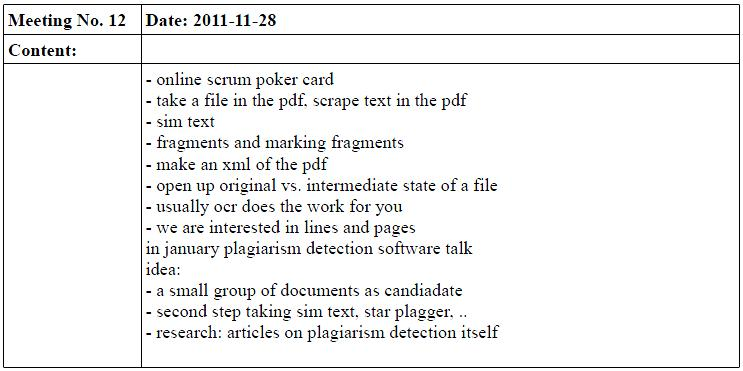
\includegraphics[width=\textwidth]{images/a_meetings/meeting_12}
  \caption{Meeting minutes no. 12}
  \label{fig:meeting minutes no. 12}
\end{figure}

\begin{figure}[htbp]
  \centering
    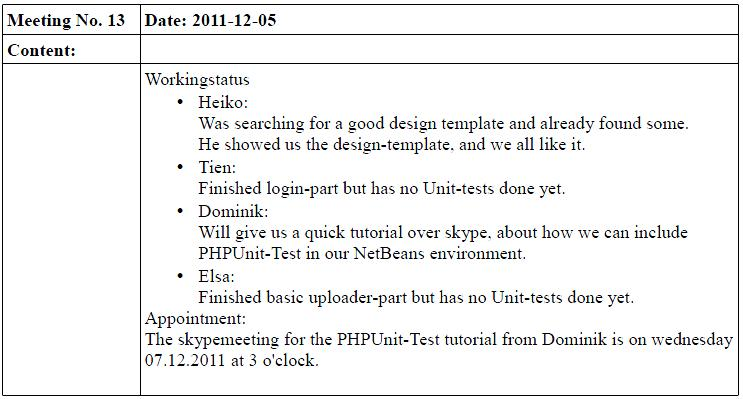
\includegraphics[width=\textwidth]{images/a_meetings/meeting_13}
  \caption{Meeting minutes no. 13}
  \label{fig:meeting minutes no. 13}
\end{figure}

\begin{figure}[htbp]
  \centering
    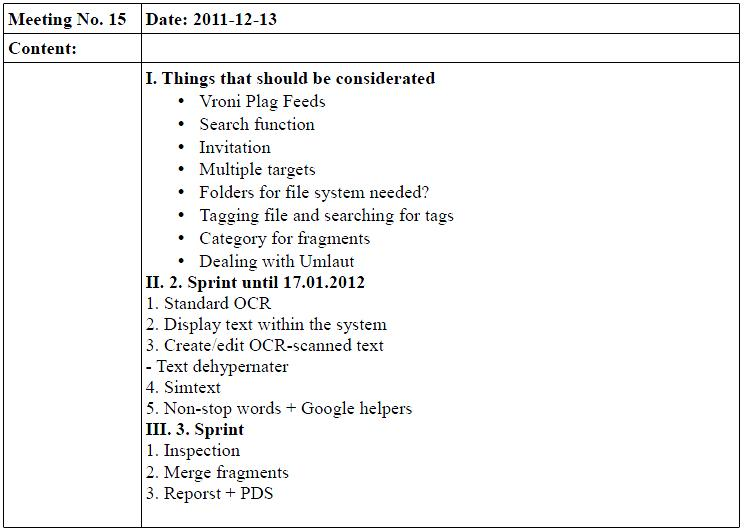
\includegraphics[width=\textwidth]{images/a_meetings/meeting_15}
  \caption{Meeting minutes no. 15}
  \label{fig:meeting minutes no. 15}
\end{figure}

\begin{figure}[htbp]
  \centering
    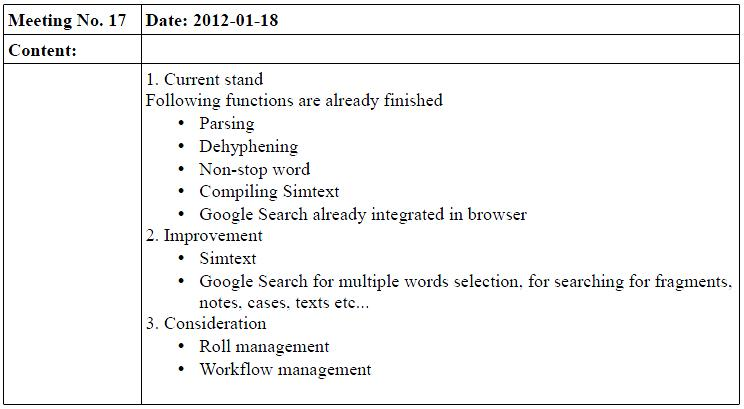
\includegraphics[width=\textwidth]{images/a_meetings/meeting_17}
  \caption{Meeting minutes no. 17}
  \label{fig:Meeting minutes no. 17}
\end{figure}

\begin{figure}[htbp]
  \centering
    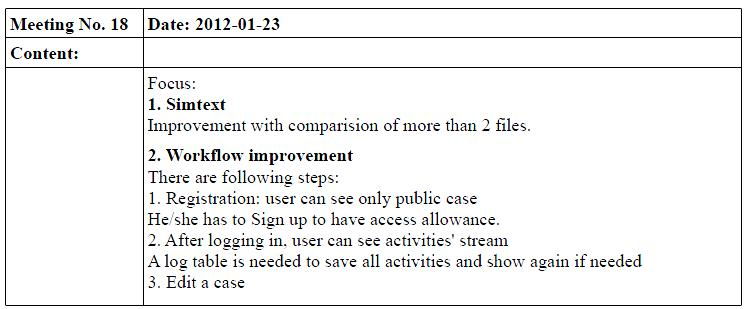
\includegraphics[width=\textwidth]{images/a_meetings/meeting_18}
  \caption{Meeting minutes no. 18}
  \label{fig:Meeting minutes no. 18}
\end{figure}

\begin{figure}[htbp]
  \centering
    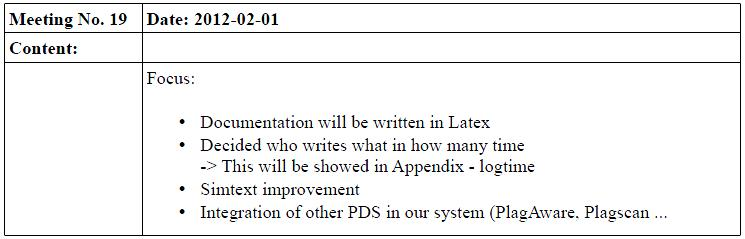
\includegraphics[width=\textwidth]{images/a_meetings/meeting_19}
  \caption{Meeting minutes no. 19}
  \label{fig:Meeting minutes no. 19}
\end{figure}

\chapter{Logged Time As Of March 22, 2012}

The following tables are some example reports generated from the logged time in Redmine. To find the most recent version
of these reports or to generate custom data analysis you can use the \enquote{Report} tool found in Redmine on the \enquote{Overview}
page.

% should be updated later on, now simply to make sure it works
% generate various reports in redmine and export as csv
% don't forget to escape special characters like _ or # in the input .csv, e. g. \_ or \#

\DTLloaddb{overview}{data/timelog-overview.csv}
\begin{table}[htbp]
  \caption{Overview By Member and Month}
  \centering
  \DTLdisplaydb{overview}
\end{table}

\begin{landscape}

\DTLsetseparator{,}

\DTLloaddb{issueMember}{data/timelog-issue-member.csv}
  \centering
 \DTLdisplaylongdb[caption=Overview By Member and Issue]{issueMember}

\DTLloaddb{sprints}{data/timelog-sprints.csv}
\begin{table}[htbp]
  \caption{Overview By Sprints}
  \centering
  \DTLdisplaydb{sprints}
\end{table}

\end{landscape}

\chapter{Mockups}\label{appendix:mockups}

\section{Hand-Drawn}

\begin{figure}[!h]
  \centering
    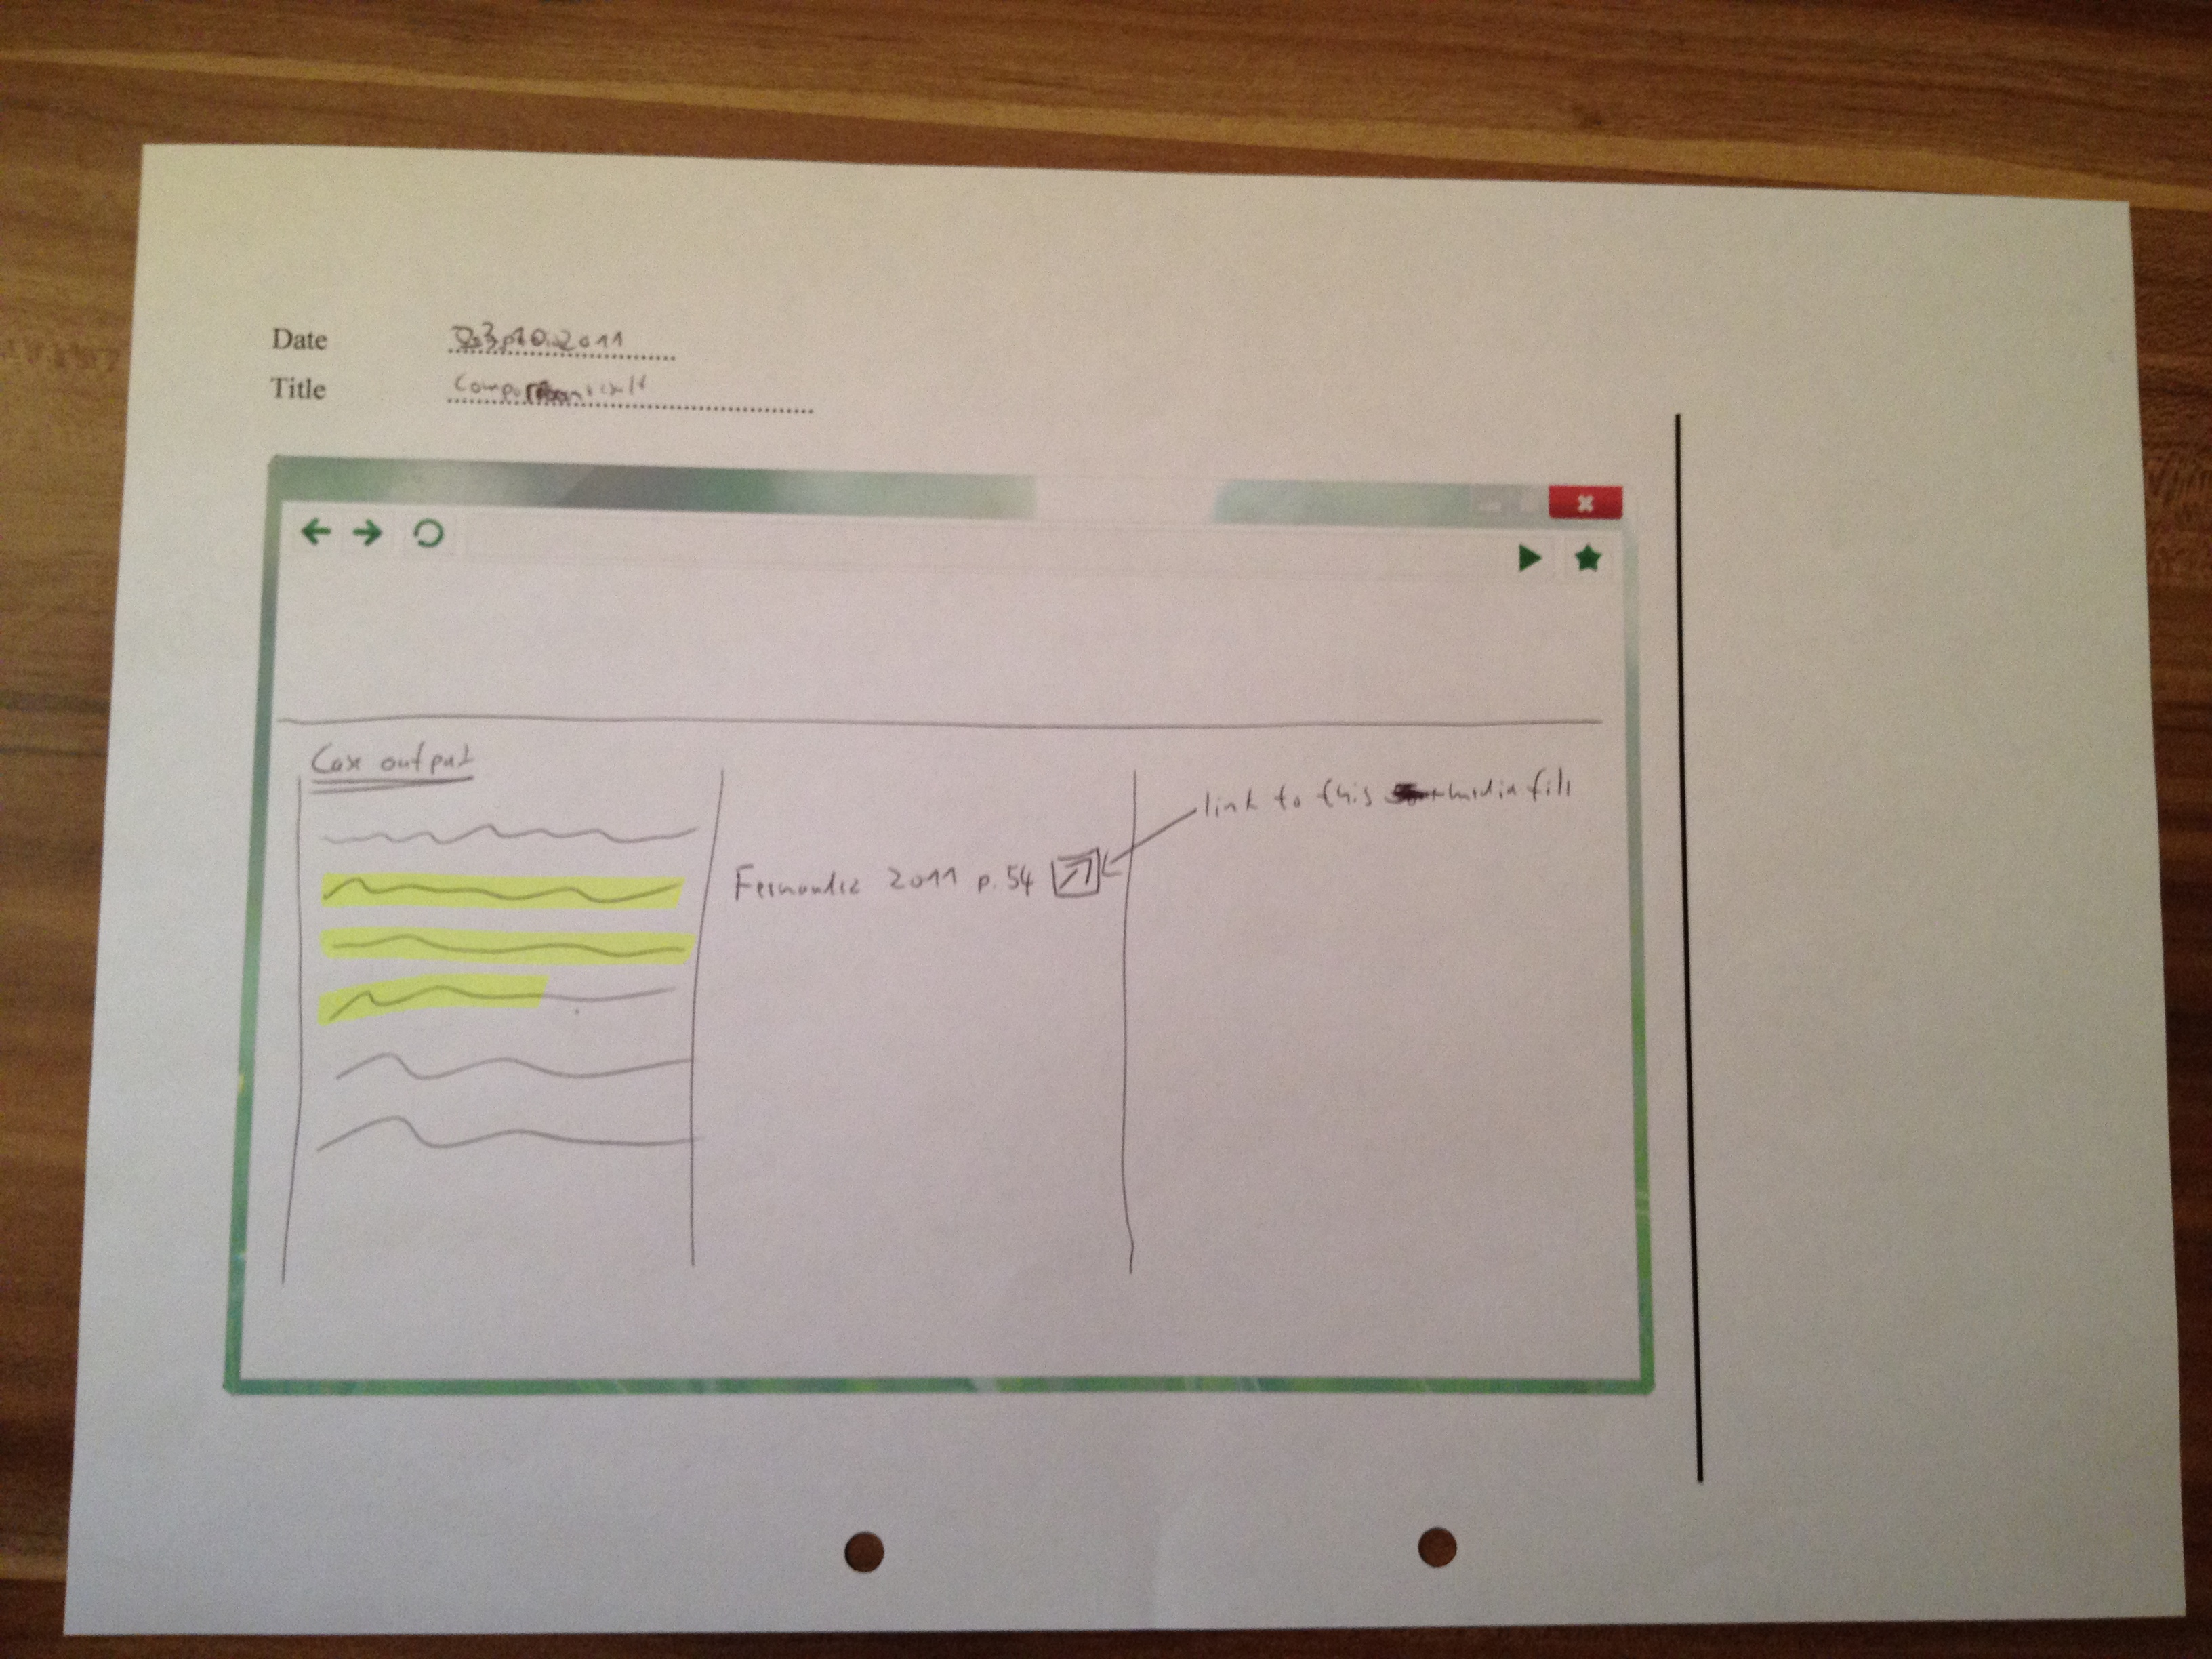
\includegraphics[width=\textwidth]{mockups/m_compare_result.jpg}
  \caption{Mockup – Compare results – digitalized }
  \label{fig:mCompareResultsMockup}
\end{figure}

\begin{figure}[!h]
  \centering
    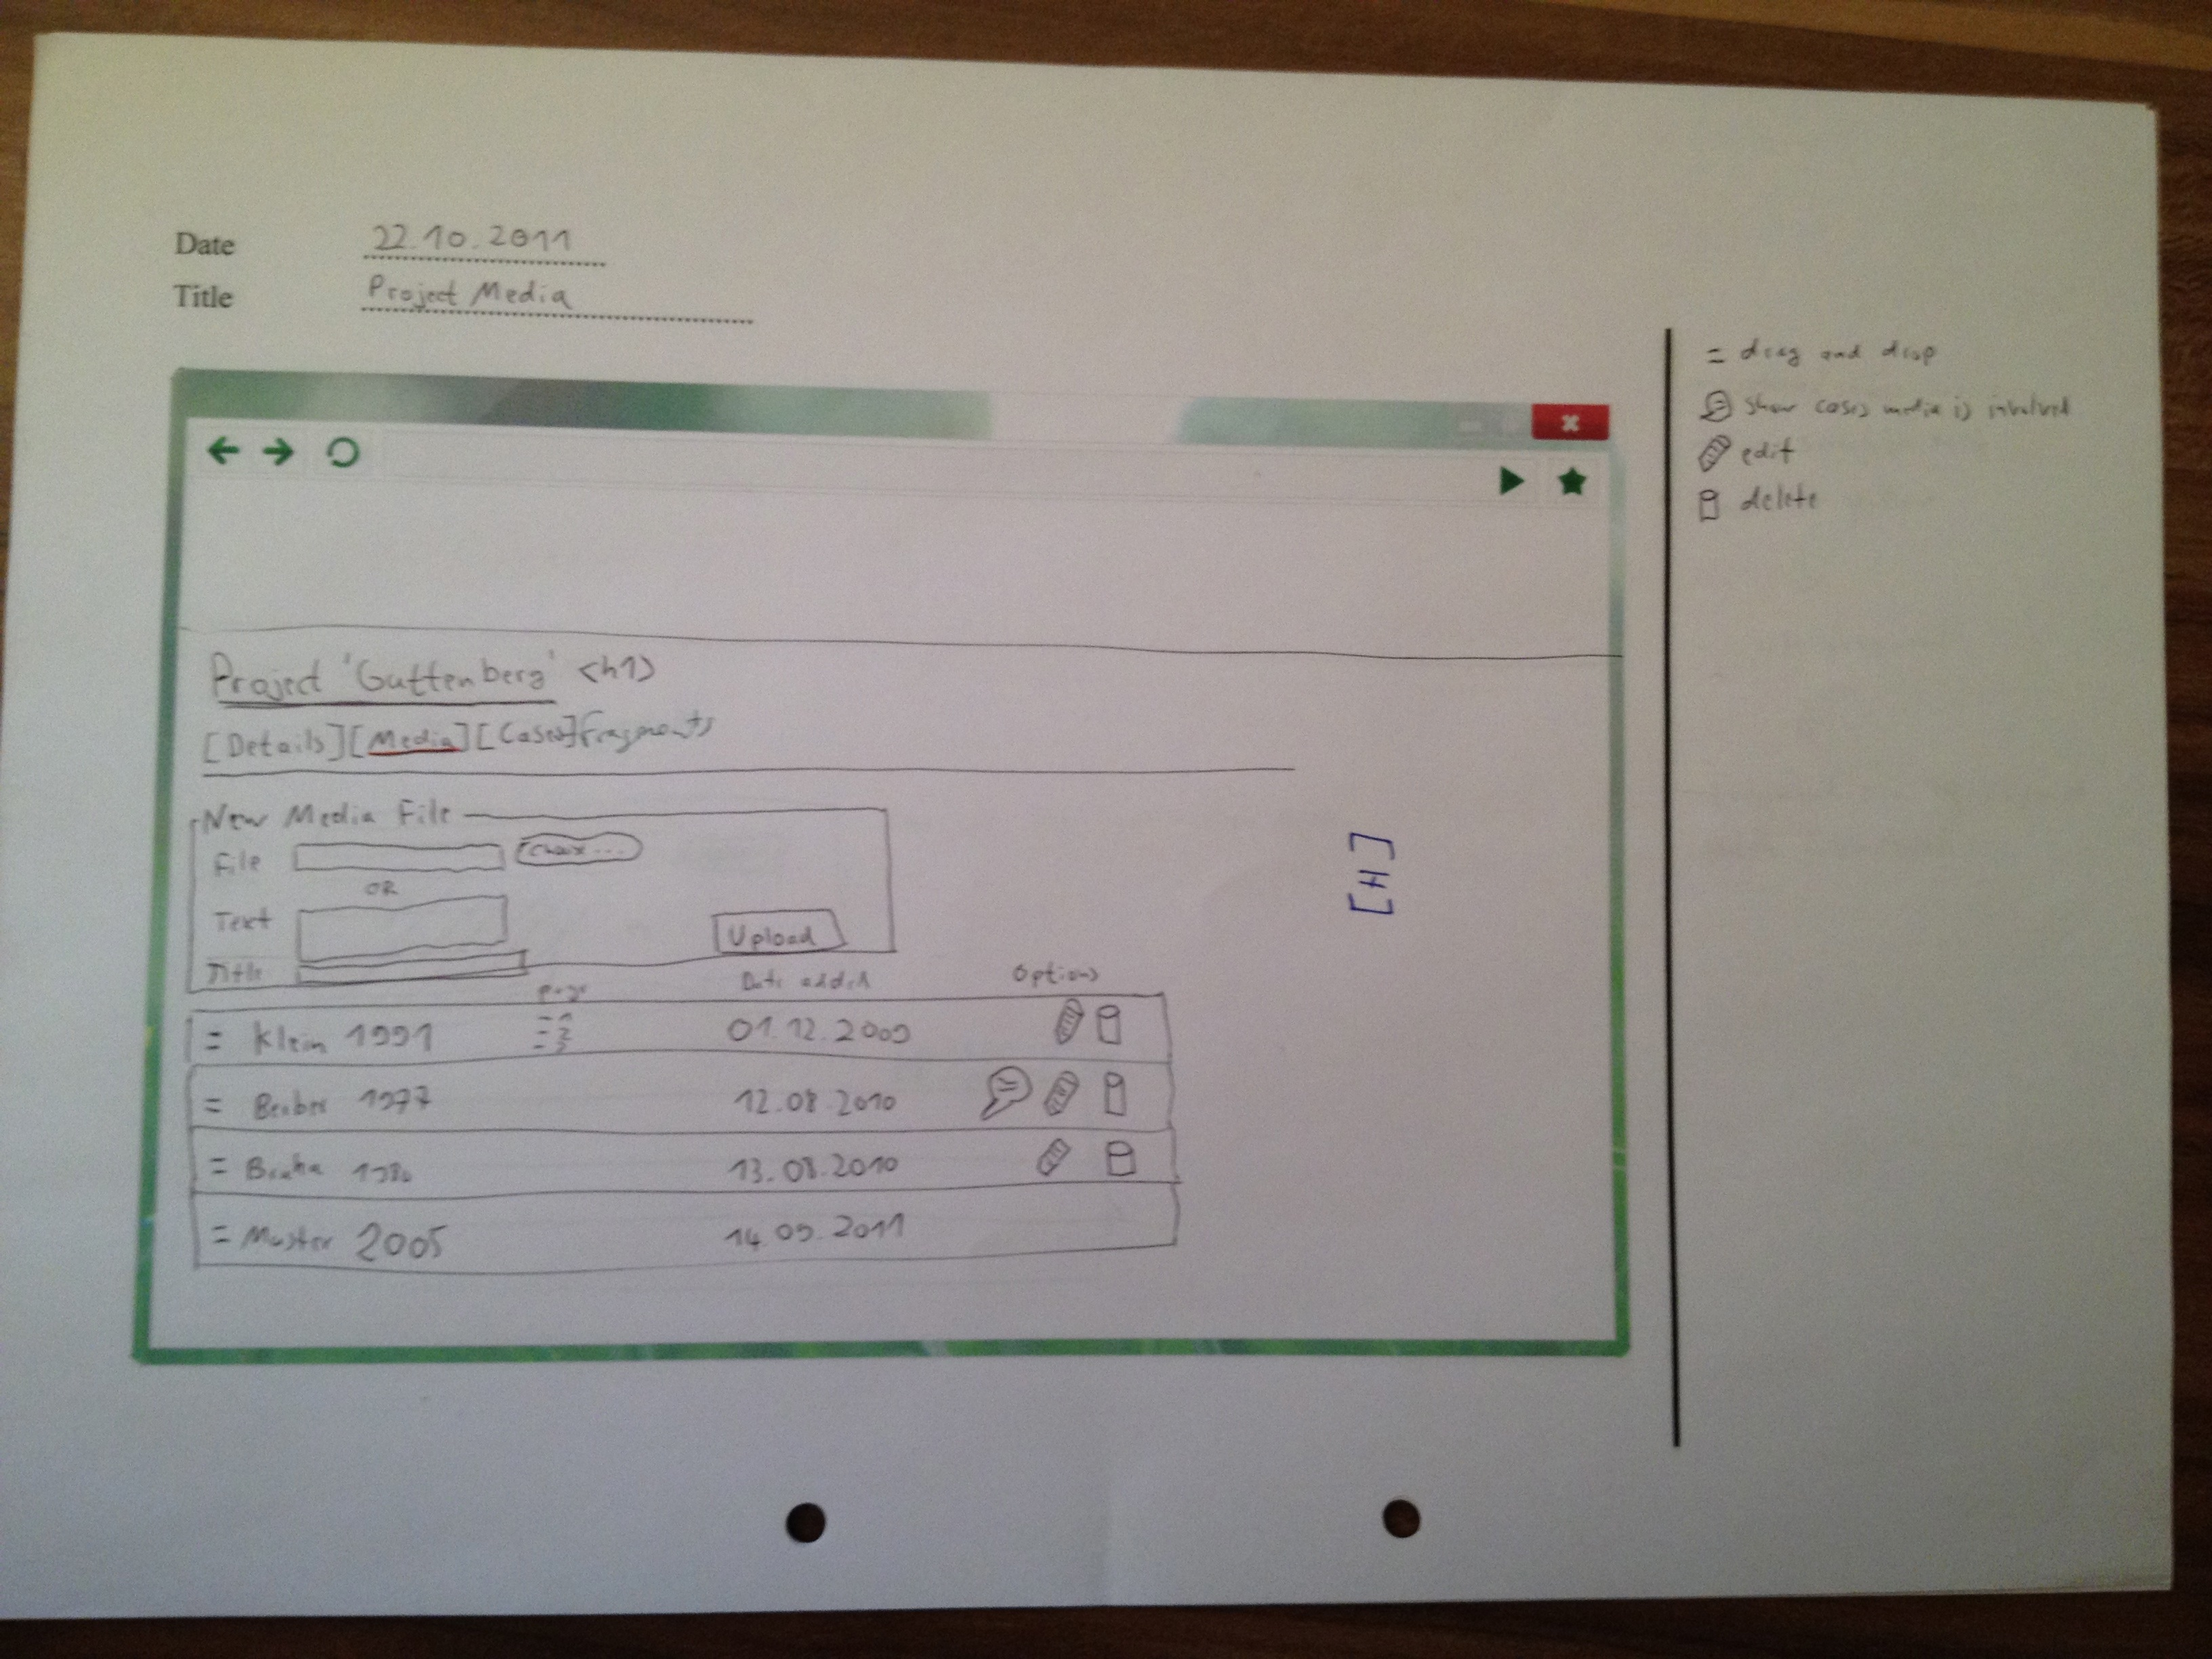
\includegraphics[width=\textwidth]{mockups/m_media_list.jpg}
  \caption{Mockup – Media list – digitalized }
  \label{fig:mMediaListMockup}
\end{figure}

\begin{figure}[!h]
  \centering
    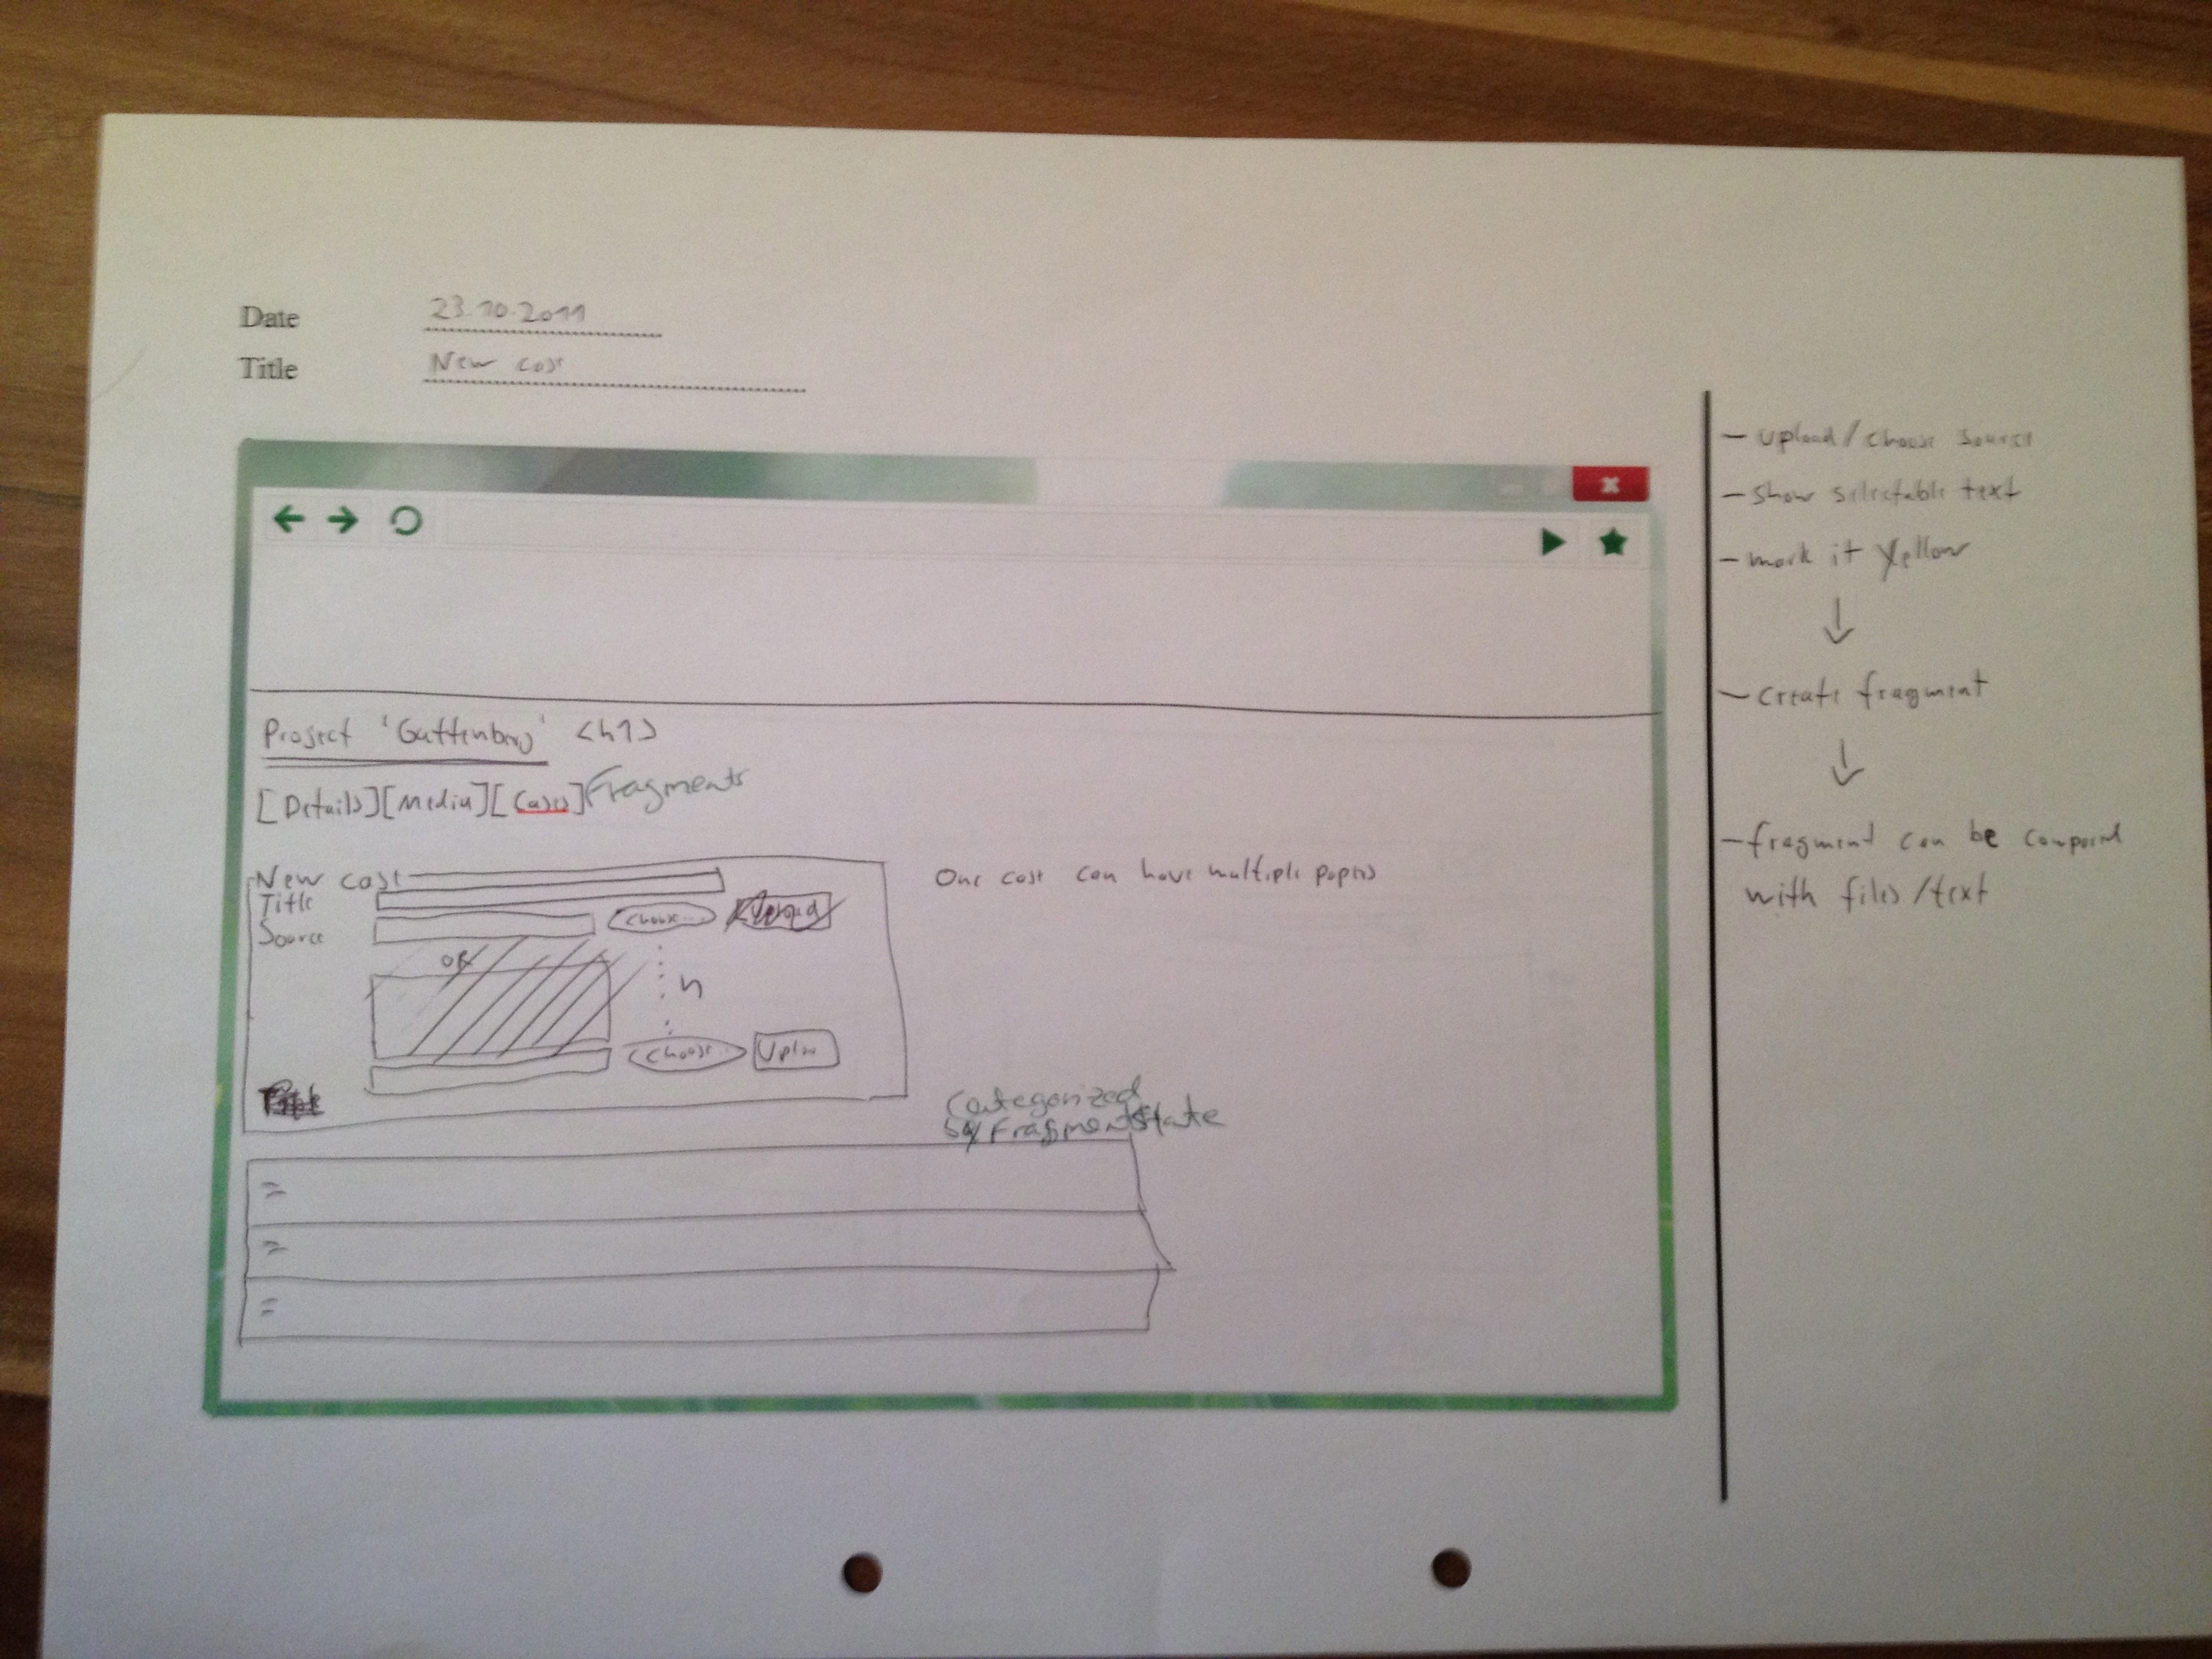
\includegraphics[width=\textwidth]{mockups/m_new_case.jpg}
  \caption{Mockup – New case – digitalized }
  \label{fig:1newCaseMockup}
\end{figure}

\begin{figure}[!h]
  \centering
    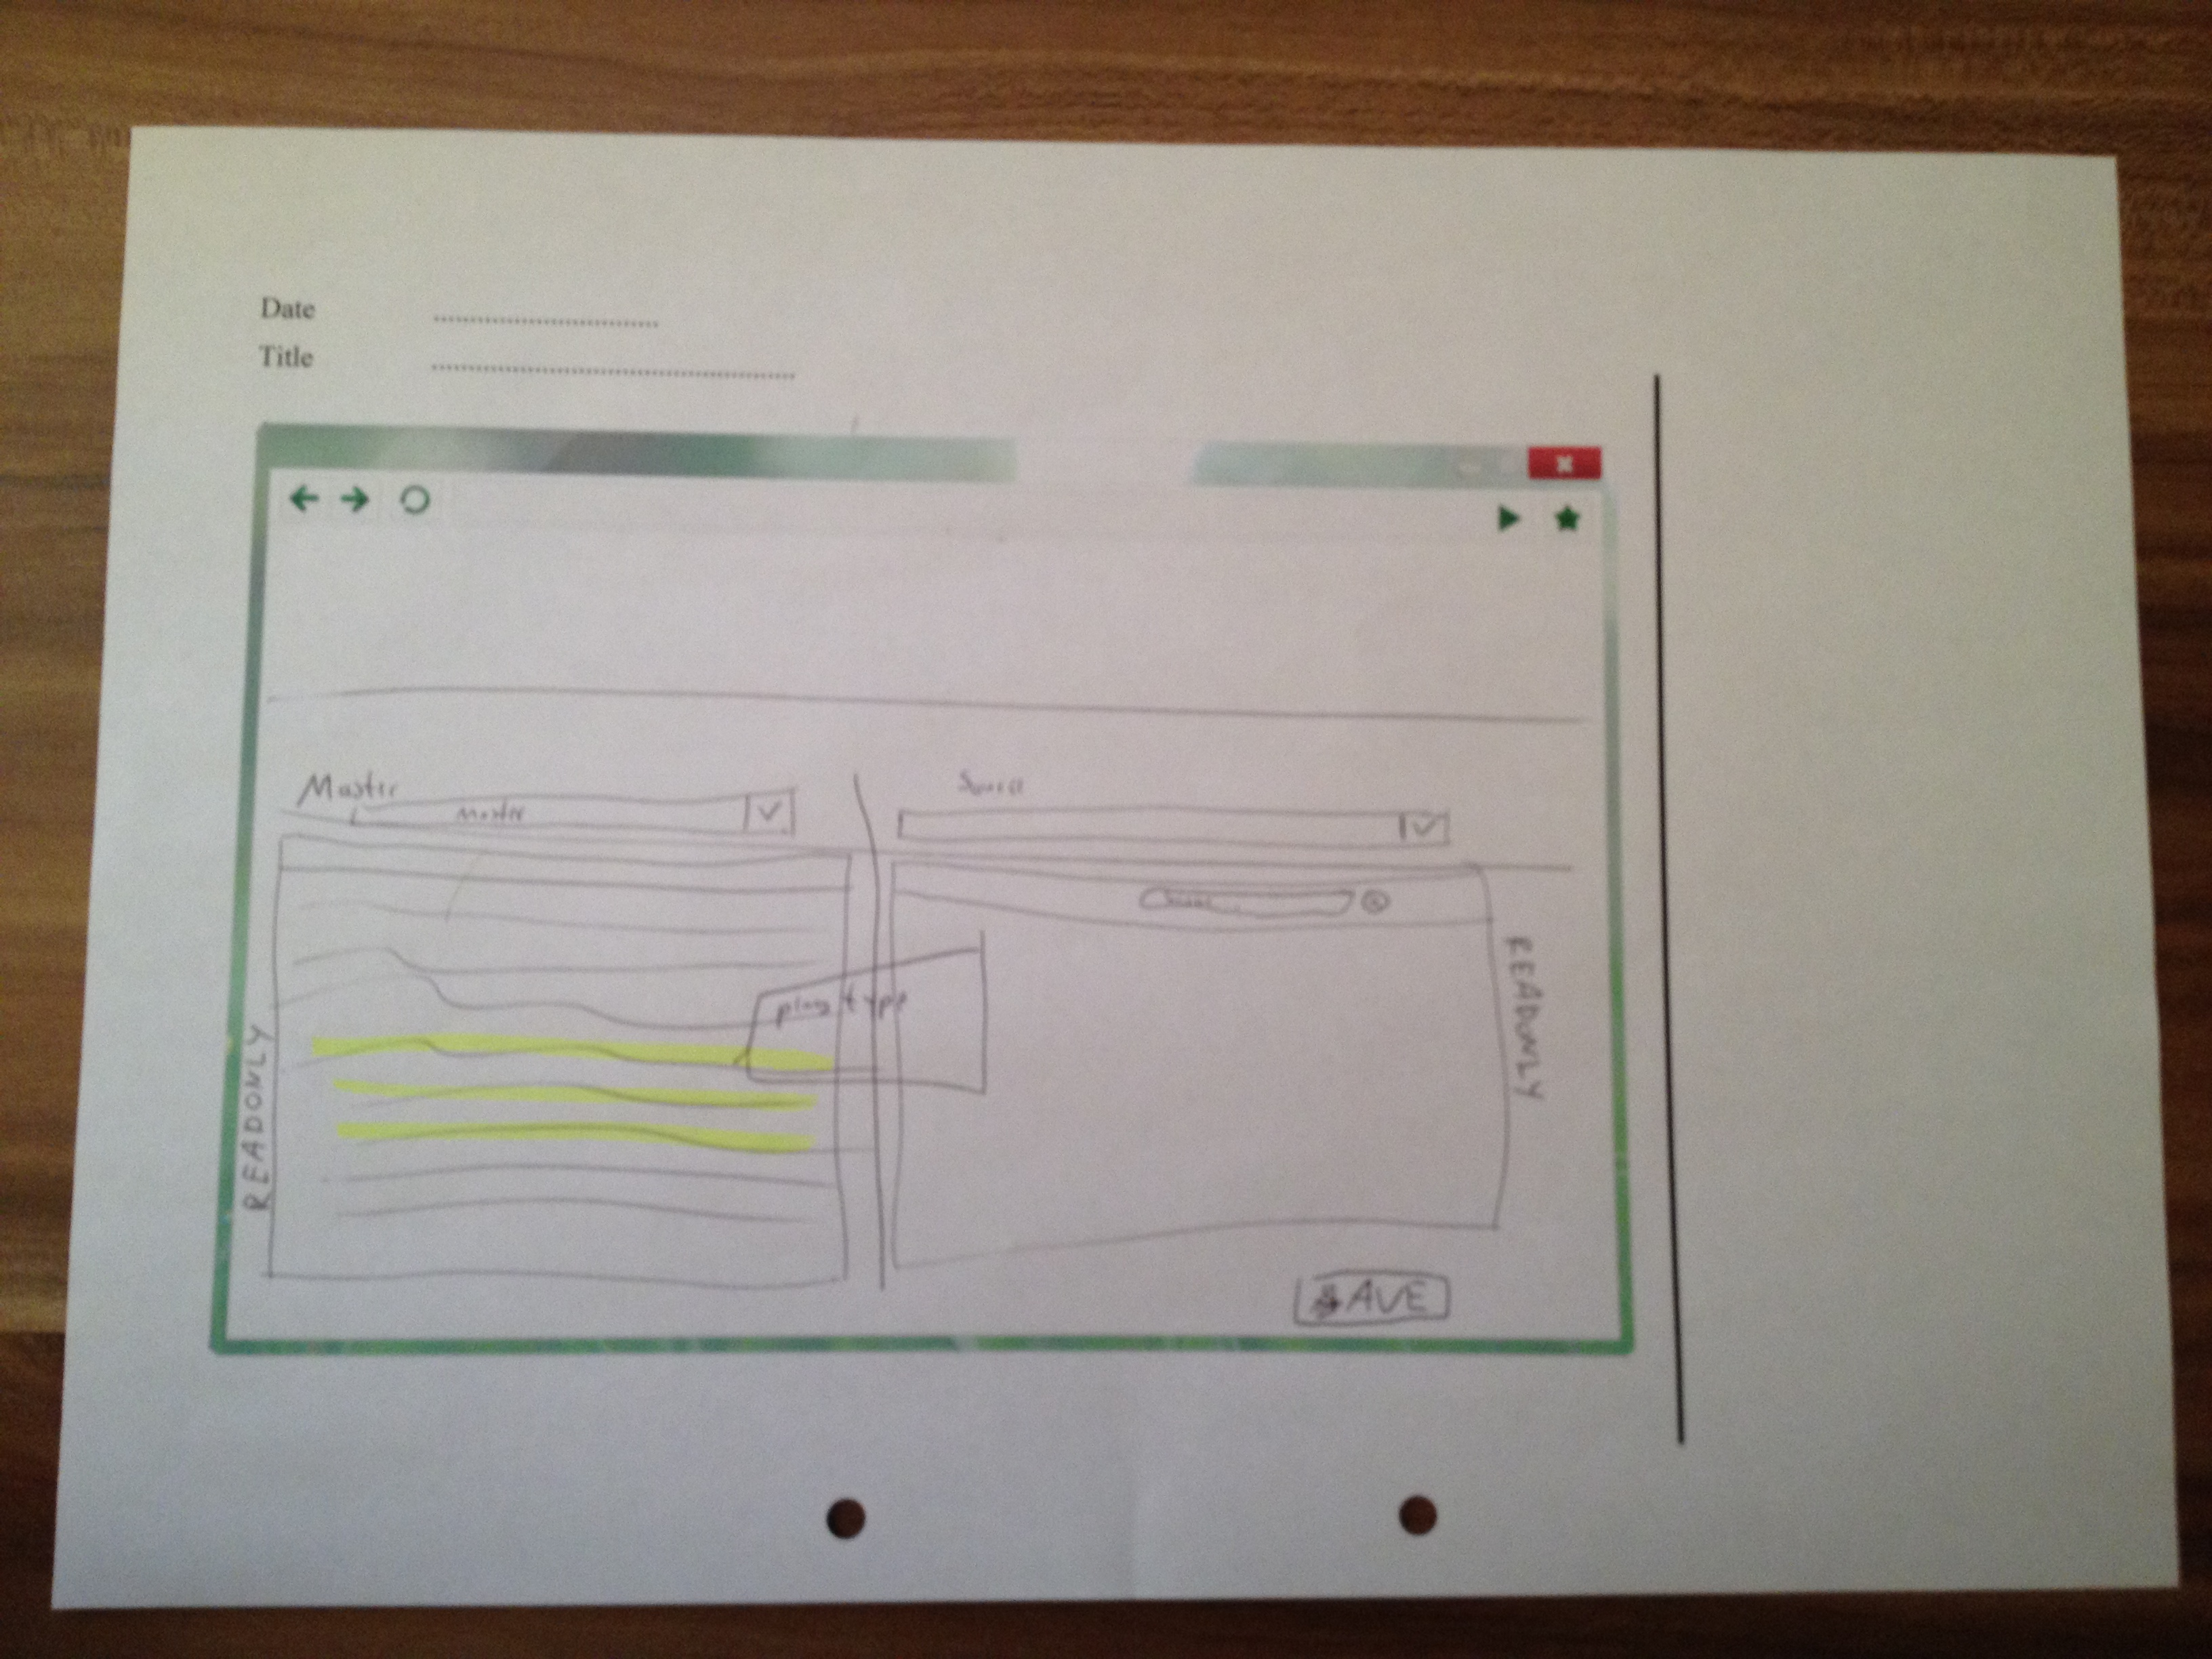
\includegraphics[width=\textwidth]{mockups/m_new_fragment.jpg}
  \caption{Mockup – New fragment – digitalized }
  \label{fig:1newCaseMockup}
\end{figure}

\begin{figure}[!h]
  \centering
    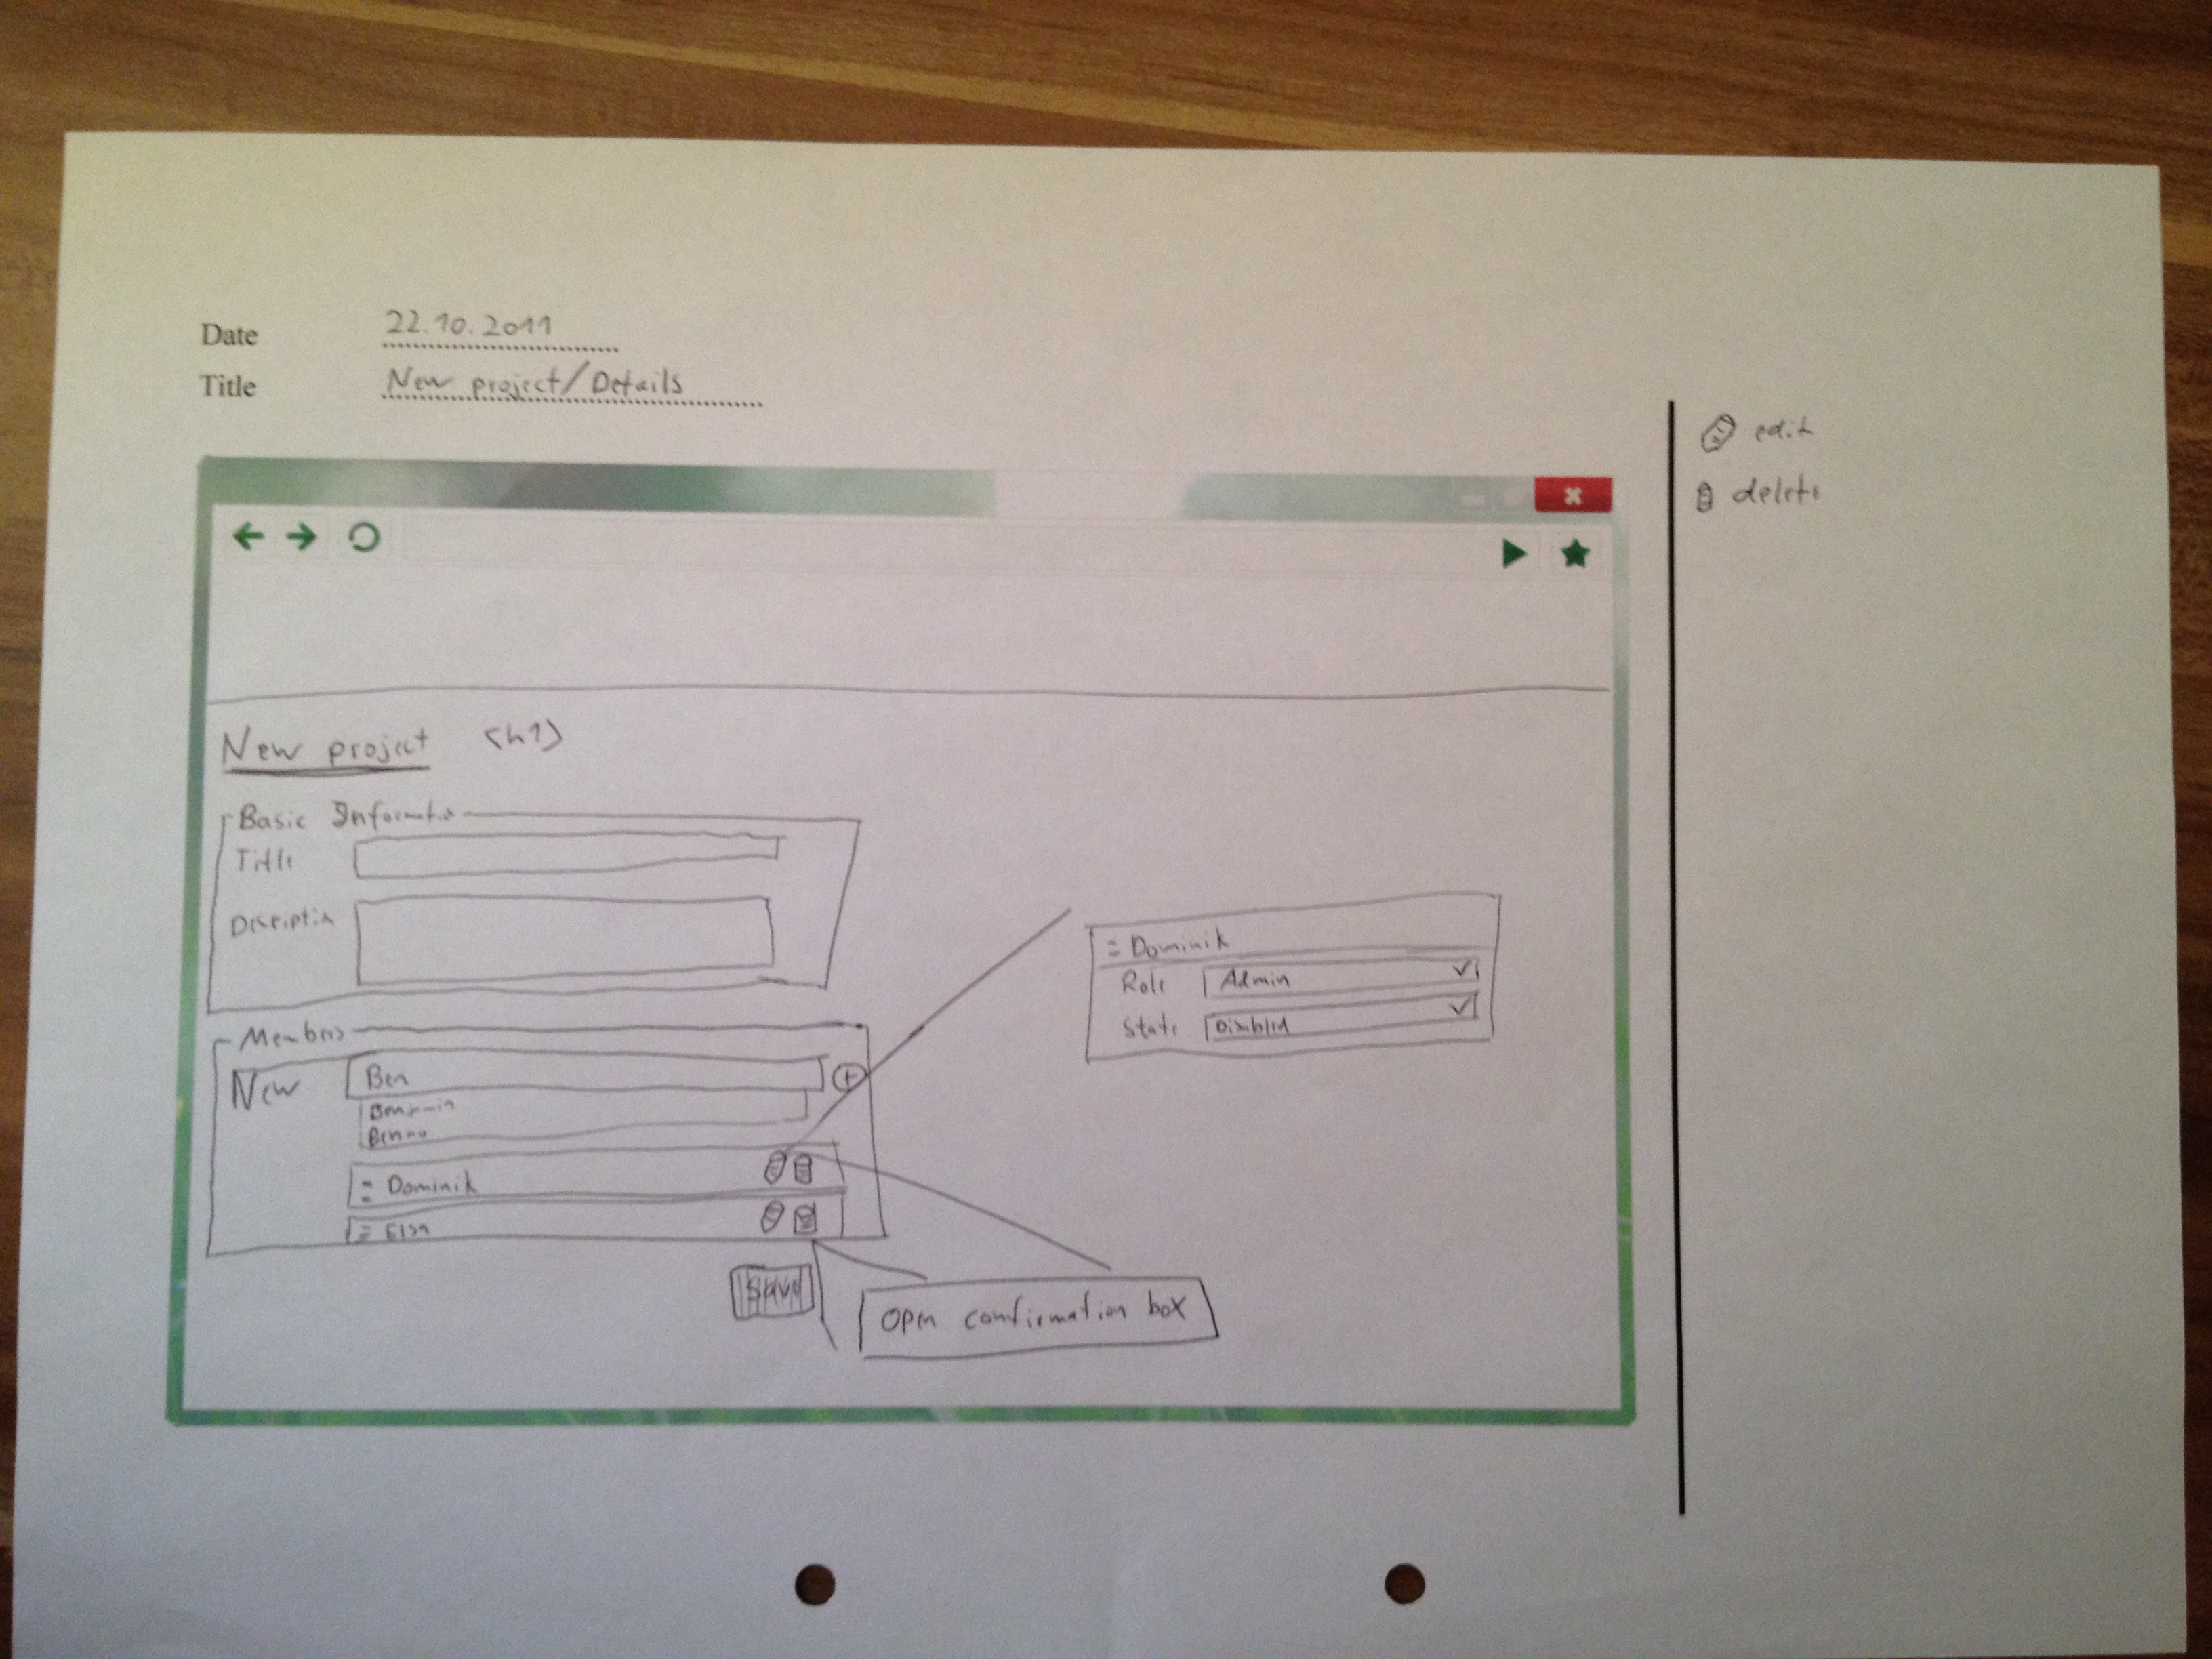
\includegraphics[width=\textwidth]{mockups/m_new_project.jpg}
  \caption{Mockup – New project – digitalized }
  \label{fig:mNewProjectMockup}
\end{figure}

\clearpage
\section{Digitalized}

\begin{figure}[htbp]
  \centering
    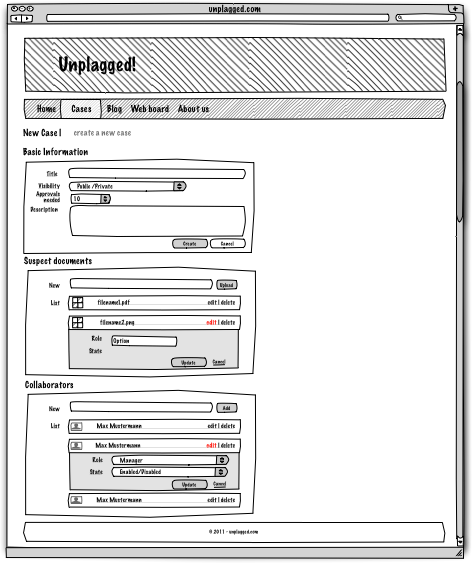
\includegraphics[width=0.86\textwidth]{mockups/1_new_case.png}
  \caption{Mockup – New case – digitalized }
  \label{fig:1newCaseMockup}
\end{figure}

\begin{figure}[!h]
  \centering
    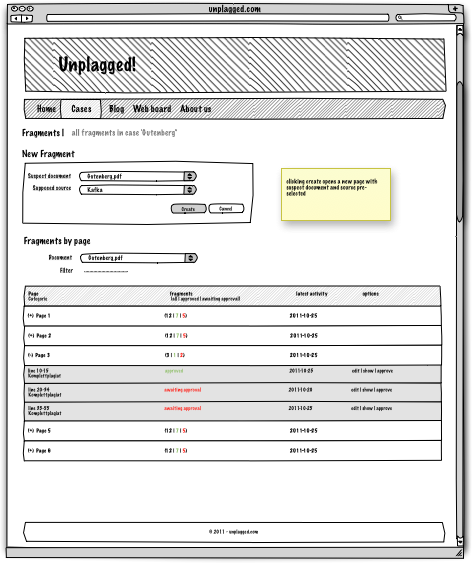
\includegraphics[width=\textwidth]{mockups/2_list_fragments.png}
  \caption{Mockup – List fragments – digitalized }
  \label{fig:2listFragmentsMockup}
\end{figure}

\begin{figure}[!h]
  \centering
    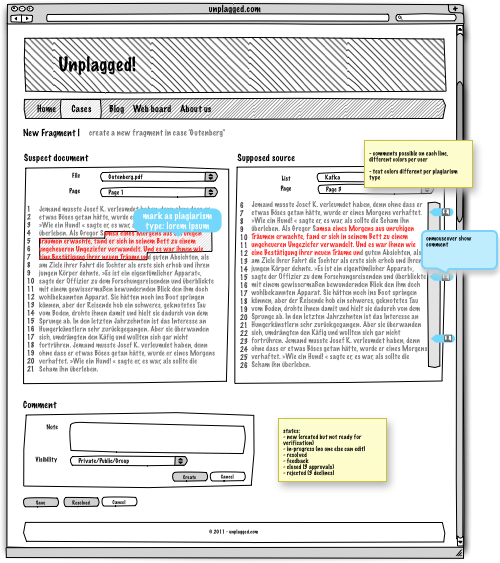
\includegraphics[width=\textwidth]{mockups/3_new_fragment.png}
  \caption{Mockup – New fragment – digitalized }
  \label{fig:3newFragmentMockup}
\end{figure}

\begin{figure}[!h]
  \centering
    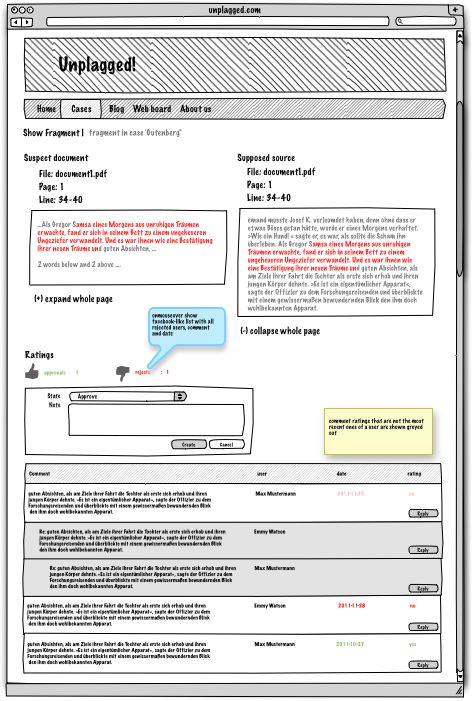
\includegraphics[width=0.97\textwidth]{mockups/4_show_fragment_for_approval.png}
  \caption{Mockup – Show fragment for approval – digitalized }
  \label{fig:4showFragmentForApprovalMockup}
\end{figure}

\begin{figure}[!h]
  \centering
    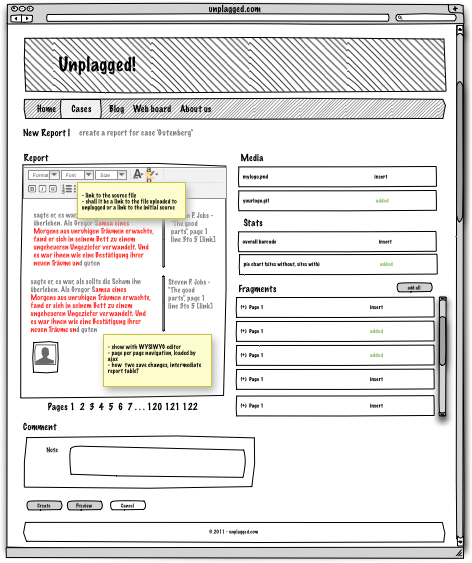
\includegraphics[width=\textwidth]{mockups/5_new_report.png}
  \caption{Mockup – New report – digitalized }
  \label{fig:5newReportMockup}
\end{figure}

\end{appendix}
